\chapter{Introduction}
\section{Centromere is a specialised locus for chromosome segregation}

 The growth and reproduction of all living organisms rely on cell division. Delivering an intact genome to the daughter cell challenges every dividing cell. Eukaryotes package their genomes into chromosomes, which must be replicated and segregated faithfully during each cell division. Severe diseases, such as cancer, genetic disorder and miscarriage, could arise if chromosome segregation is compromised \citep{Jallepalli2001ChromosomeMystery, Draviam2004ChromosomeStability, Wasielak-Politowska2022ChromosomeAging, Losada2014CohesinBeyond}. 
 
 Centromere is the specialised locus for chromosome segregation, where the chromosome is attached to and pulled by the spindle \citep{Westhorpe2015AMaintenance, McKinley2015TheFunction, Talbert2020WhatCentromere, Fukagawa2014}. First described by \cite{Flemming1882ZellsubstanzZelltheilung} as primary constriction, it is visualised as the intersection point of the iconic X-shaped mitotic chromosome under a microscope. Lack of centromere, or being acentric, leads to chromosome loss during cell division. Although the appreciation of centromere function has been established since its discovery, the molecular feature underneath remained elusive due to the species-to-species variations and the complexity of players involved. \cite{Darlington1936TheEnquiry} therefore recommended defining the centromere in terms of the function rather than the form. Nevertheless, advances in molecular biology shed light on the form of centromere. In most species, the centromeric DNA sequence plays an important but not definitive role in centromere specification \citep{Hoffmann2020, Harrington1997FormationMicrochromosomes, Catania2015SequenceChromatin, Iwata-Otsubo2017, Kasinathan2018Non-B-FormCentromeres, Shukla2018CentromereCycle, Logsdon2019, Murillo-Pineda2020}. It is instead determined epigenetically by the histone H3 variant CENP-A \citep{Warburton1997ImmunolocalizationCentromeres, Vafa1997ChromatinPlate, Earnshaw1985ThreeChromosome, Liu2006MappingCells, Regnier2005CENP-ABubR1, Heun2006, Mendiburo2011, Barnhart2011, Logsdon2015}. The macromolecular protein complex consisting of around 100 subunits, kinetochore, is formed on the centromere to mediate the physical connection between the chromosome and spindle microtubules and act as a signalling hub to monitor the interaction \citep{Musacchio2017AFunction, McAinsh2022TheKinetochores, Cheeseman2014TheKinetochore, Hara2018KinetochoreExit}. Apart from the progress in the form, the mechanisms centromere executing the function have also been elucidated over the years \citep{Tanaka2013, Zhou2020EmergentChromosomes}. In the following sections, the form and function of the centromere will be described in more detail. 

\section{The form of centromere}
\subsection{The genetics}

The structure of centromeric DNA and its functional importance varies dramatically between species. Based on the chromosomal distribution, centromeres are classified as monocentromere, where the centromere is localised at a restricted region of the chromosome, and holocentromere, where the centromere spreads the entire length of the chromosome. Depending on size, the monocentromere can be further divided into point centromere, which contains a short DNA sequence of just over 100 bp, and regional centromere, which could be up to megabases long. The importance of underlying DNA sequences to centromere function could also be very different, ranging from pure genetic to mainly epigenetic. 

Point centromere, with a notable example budding yeast \textit{Saccharomyces cerevisiae}, is the simplest form and the first investigated at the molecular level. A budding yeast centromere consists of three elements \citep{Carbon1984StructuralCEN3}: CDEI, an 8-bp sequence that binds Cfb1 for H3 nucleosome eviction \citep{Niedenthal1993Cpf1I, Henikoff2011EpigenomeResolution}; CDEII, an AT-rich, around 80-bp sequence accommodating a single centromeric nucleosome containing Cse4, the budding yeast CENP-A, for kinetochore assembly \citep{Furuyama2007CentromereYeast, Henikoff2014TheVivo, Krassovsky2012TripartiteYeast} and CDEIII, a 25-bp sequence bound by the CBF3 complex \citep{Yan2018ArchitectureKinetochore}, which recruits the Cse4 chaperon Scm3, the budding yeast HJURP, for Cse4-containing nucleosome deposition \citep{Stoler2007Scm3Localization, Camahort2007Scm3Kinetochore}. Centromere specification is strictly genetic in this organism \citep{Clarke1980IsolationChromosomes, J1986SingleCerevisiae, Kingsbury1991Centromere-dependentVitro}, which could be explained by its unique centromere biology that factors for Cse4 nucleosome deposition are recruited by specific DNA sequences. This is in line with the observation that the exact sequences of CDEI and CDEIII are conserved across all 16 centromeres of budding yeast \citep{Clarke1998Centromeres:Eukaryotes, Baker2005GeneticCerevisiae}. As for the centromeric nucleosome accommodating sequence CDEII, only the length and AT abundance are conserved, supporting the notion from regional centromeres that CENP-A nucleosome binding does not require specific DNA sequences \citep{Bensasson2011EvidenceCentromeres}. The phylogeny indicated that point centromere species evolved from regional centromere species and this transition coincided with the emergence of 2-micron plasmid, a multicopy circular DNA capable of self-propagating in budding yeast \citep{Malik2009MajorComplexity}. Intriguingly, the 2-micron plasmid also uses a single locus called \textit{STB} to assemble a partitioning complex, which includes components of segregation machinery for normal chromosomes such as Cse4 and cohesin, for its association with the spindle microtubule \citep{Rizvi2018TheCerevisiae, Huang2011Evolution, Ghosh2007FaithfulSisters}. The outstanding resemblance led to the hypothesis that the point centromere is the domestication of the self-propagating locus of parasitic plasmids \citep{Malik2009MajorComplexity}. 

The regional centromere is the most common type of centromere. A typical regional centromere is AT-rich and possesses a modular structure composed of a CENP-A-nucleosome-accommodating central core flanked by heterochromatic domains called peri-centromere. The central core usually contains satellite DNA, short sequences repeated a large number of times, whereas the peri-centromere has less patterned sequences \citep{Talbert2020WhatCentromere, McKinley2015TheFunction, Wong2020LessonsChromosomes, Muller2019TheArchitecture}. As one of the fastest-evolving loci across the genome, the precise sequence of the centromere is extremely diverse among species \citep{Melters2013ComparativeEvolution}. Notably, due to the incompatibility of second-generation sequencing and repetitive sequence, deciphering the centromeric DNA sequence has been challenging. In fission yeast \textit{Schizosaccharomyces pombe}, the central core consists of non-repetitive \textit{cc} and inverted repeats \textit{imr} while the peri-centromere possess less ordered \textit{otr} composed of \textit{dg} and \textit{dh} repeats \citep{Chikashige1989CompositeSites, Clarke1993StructureCentromeres, Murakami1991StructureRegion, Nakaseko1986ChromosomeYeast, Nakaseko1987AChromosomes., Steiner1993CentromeresLoci}. Fruit fly \textit{Drosophila melanogaster} has a central core made up of a retroelement-enriched island flanked with AATAT and AAGAG satellites, and peri-centromeric chromatin containing mixed different types of short satellites that are neither conserved among chromosomes nor specific to the centromere \citep{Talbert2018SimpleSpecies, Wong2020LessonsChromosomes, Chang2019IslandsCentromeres}. House mouse \textit{Mus musculus} centromeres are close to telomeres, which is termed acrocentric. The central core and the peri-centromere consist of 120-bp minor satellites and 234-bp major satellites, respectively \citep{Komissarov2011TandemlyGenome, Kuznetsova2006High-resolutionDNA}. Primate including human \textit{Homo sapiens} central core contains 171-bp monomers, named $\alpha$-satellite, arranged into HOR arrays of different lengths, whereas the flanking peri-centromere is built with less structured monomeric $\alpha$-satellites that are less recognisable \citep{Maio1971DNAAethiops, Rosenberg1978HighlySIMIANSIMIANSIMIANSIMIANSIMIAN, Manuelidis1978ComplexDNAs, Manuelidis1978ChromosomalDNAs, Aldrup-MacDonald2014TheGenomics, Logsdon2021The8}. Unlike the point centromere, the centromeric DNA sequence is neither sufficient nor necessary for the function of the regional centromere \citep{McKinley2015TheFunction}. The former was indicated by the observations that the dicentric chromosomes due to the fusion of two normal chromosomes only assembled centromeric proteins, such as CENP-A, at one of the two endogenous centromeres \citep{Earnshaw1985ThreeChromosome, Steiner1994AYeast, Higgins2005EngineeredPlasticity, Sato2012EpigeneticChromosomes, Sullivan1995IdentificationCentromeres, Lange2009IsodicentricPalindromes}. The latter was evidenced by the fact the ectopic centromere, neocentromere, can form on chromosomal regions whose sequences bear little similarity with the canonical centromeres \citep{Marshall2008Neocentromeres:Evolution, Voullaire1993ACentromere, Tyler-Smith1999TransmissionGenerations, Amor2004HumanProgress}. The epigenetic notion was later confirmed by the elucidation of the requirement of CENP-A for centromere function and localisation \citep{Warburton1997ImmunolocalizationCentromeres, Vafa1997ChromatinPlate, Liu2006MappingCells, Regnier2005CENP-ABubR1, Heun2006, Mendiburo2011, Barnhart2011, Logsdon2015, Logsdon2019}. However, experimental results that cloned regional centromeric sequences were sufficient to support the inheritance of exogenous DNA suggest a contribution of sequence to \textit{de novo} centromere formation \citep{Hahnenberger1989ConstructionPombe., Haaf1992IntegrationSegregation, Harrington1997FormationMicrochromosomes, Ikeno1998ConstructionChromosomes}. This could partially be explained by the presence of the sequence-specific DNA-binding centromeric protein CENP-B \citep{Masumoto1989ASatellite., Muro1992CentromereBox., Earnshaw1985IdentificationScleroderma}. CENP-B is not essential for the centromere function as evidenced by that CENP-B knockout mice are still viable \citep{Kapoor1998TheMice, Perez-Castro1998CentromericAbnormalities, Hudson1998CentromereWeights}. But the centromere of the Y chromosome, which lacks CENP-B binding sequences called CENP-B box, failed to generate HACs \textit{in vivo} \citep{Harrington1997FormationMicrochromosomes, Grimes2002-SatelliteFormation}, consistent with the idea that centromeric DNA sequences facilitate the establishment of a functional centromere. The molecular mechanism was later uncovered that CENP-B interacts with both CENP-A and the CCAN component CENP-C to facilitate CENP-A deposition and kinetochore assembly \citep{Chardon2022CENP-B-mediatedCentromeres, Fachinetti2013, Fachinetti2015, Fujita2015StableNucleosome}. As mentioned above, the repetitiveness of centromeric sequences is a conserved feature in various regional centromere species and therefore evolutionarily preferred. Moreover, newly positioned centromeres from speciation, the ENCs, tend to gradually acquire repetitive sequences over time \citep{Rocchi2011CentromereMammals, Kasai2003ChromosomeEvolution}. The hypothesised mode of action is that younger sequences were inserted at the central core, pushing the old sequences towards the flank \citep{Locke2011ComparativeGenomes, Piras2010UncouplingEquus, Ventura2001CentromereEvolution, Kalitsis2012TheCentromere}, which was supported by the recently revealed complete human centromere sequences \citep{Logsdon2021The8}. The evolutionary preference for repetitive sequences also implied its importance to centromere function. It is speculated that tandem repeats might prevent the CENP-A domains from sliding along the centromere over cell cycles \citep{Nergadze2018BirthDomains}. 

Holocentromere refers to the situation where a diffused centromere extends along the whole length of the chromosome instead of a localised one \citep{Guerra2010NeocentricsRules}. It is often seen in flowering plants, insects, arachnids, and nematodes, including the model organism roundworm \textit{Caenorhabditis elegans} \citep{Wong2020LessonsChromosomes}. In mitosis, the holocentromere resides at the poleward faces of the chromosome whereas there is less of a common feature for meiosis \citep{Maddox2004HoloerElegans, Buchwitz1999AElegans, Marques2016HolocentromereHolocentromeres}. At the DNA sequence level, satellites and retrotransposons are enriched in the genome of holocentromere species but they lack an outstanding pattern as in regional centromere species \citep{Kang2016DifferentialElimination, Heckmann2013TheOrganization, Marques2016RestructuringPubera}. In beak-sedge \textit{Rhynchospora pubera} and \textit{C. elegans}, CENP-A nucleosomes do indicate a preferred association with certain DNA sequences \citep{Marques2016HolocentromereHolocentromeres, Gassmann2012AnElegans, Steiner2014HolocentromeresHotspots}. But the fact that these sequences are also actively transcribed suggests the possibility that CENP-A nucleosomes are preferentially loaded at these sites due to their accessibility created by the transcription factors. Indeed, when assessing the importance of DNA sequences for centromere formation in \textit{C. elegans}, it was found that the inheritance of WACs and generation of functional holocentromeres were independent of the DNA sequences used \citep{Stinchcomb1985ExtrachromosomalElegans, Yuen2011RapidEmbryos}. Interestingly, holocentromere has emerged multiple times independently in evolution, termed as convergent evolution in Genetics \citep{Guerra2019MonocentricFamily, Drinnenberg2014RecurrentInsects, Melters2012HolocentricAnalysis}, suggesting a selective force favouring the phenotype. It is unclear what the driver is but one hypothesis is that holocentromere can prevent the loss of fragmented chromosomes due to ionising radiation \citep{Zedek2018HolocentricLand}. Besides the three types of centromere mentioned above, there exists another variety where a few large distinct centromeric domains co-exist on a chromosome, called meta-polycentromere, which is recognised as the intermediate of holocentromere evolution \citep{Neumann2012StretchingDomains}. 

\begin{figure}[htbp]
  \centering
  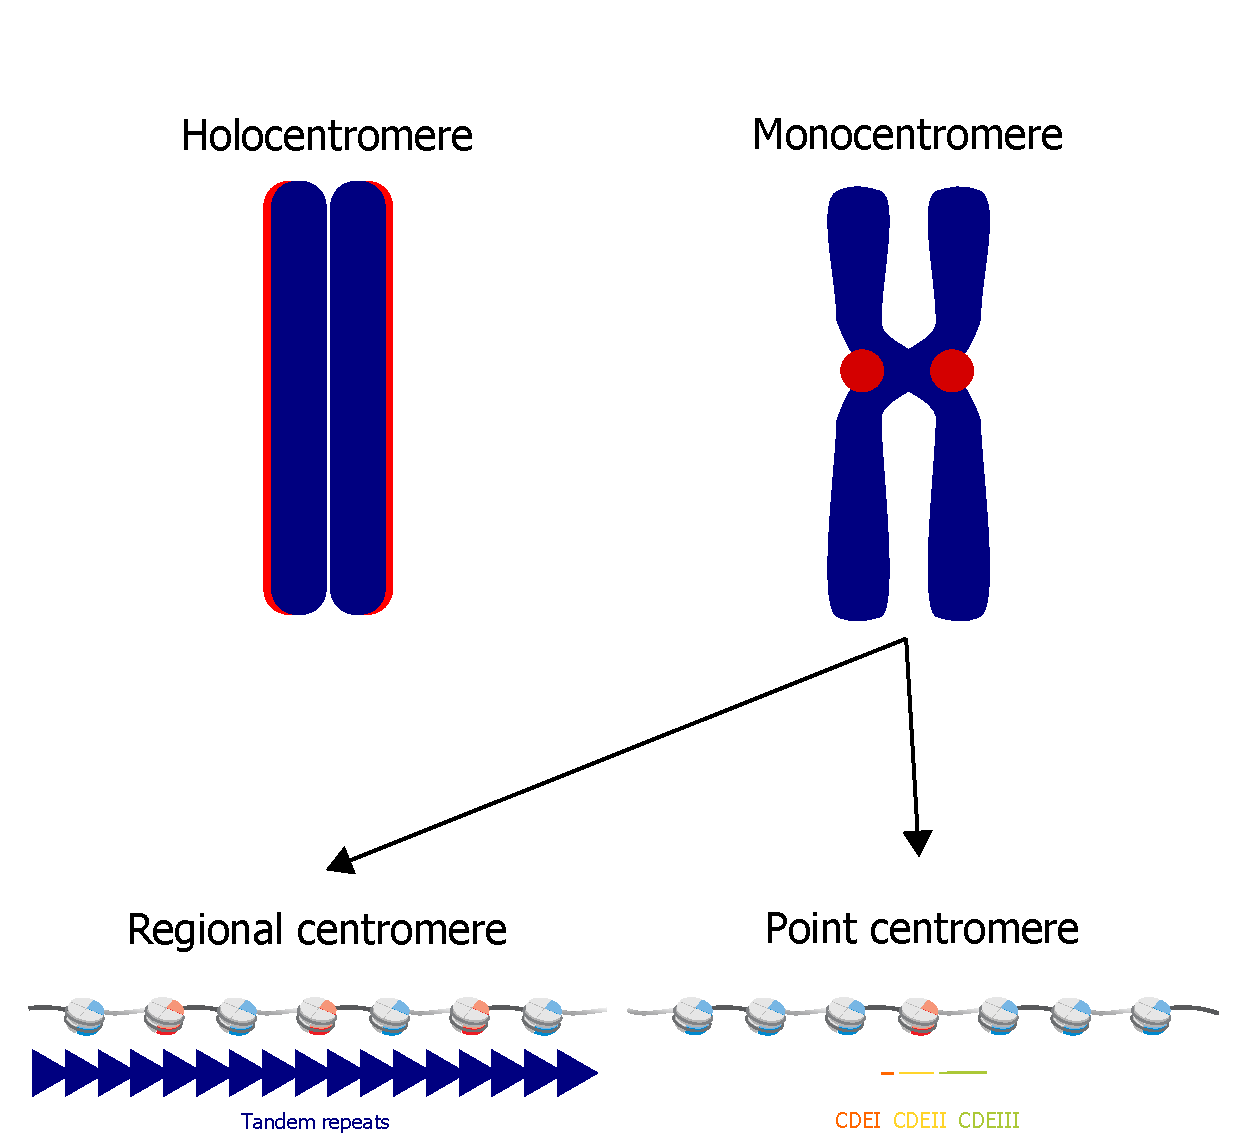
\includegraphics[width=0.9\textwidth]{chapter1/figures/centromere types.pdf}
  \caption[Different types of centroemres]{Different types of centroemres. Broadly, centromeres can be classified into holocentromere or monocentromere, depending on whether a diffused or localised centromere (red) is assembled on the chromosome (blue) under a microscope. Based on the length of DNA sequences and the number of CENP-A nucleosomes, monocentromere can be further divided into regional centromere or point centromere. A regional centromere usually possesses repetitive DNA sequences up to megabases in length and a large number of CENP-A nucleosomes. A point centromere is only composed of over 100 bp DNA sequences and one single CENP-A nucleosome. }
  \label{fig:cenTypes}
\end{figure}

Another common feature of centromeric DNA is the presence of non-B form DNA \citep{Kasinathan2018Non-B-FormCentromeres}, which refers to DNA structures other than the canonical one, such as hairpins and i-motifs. The former has been observed in humans, \textit{Drosophila melanogaster}, old-world monkeys and budding yeast while the latter has been seen in \textit{Drosophila dodeca} and humans \citep{Koch2000NeocentromeresDNA, Ferrer1995CentromericStructures, Catasti1994UnusualCentromeres}. <10-bp dyad symmetries found in many organisms are thought to be responsible for the formation of non-B form DNA. Notably, it is not the case for great apes and mice \citep{Kasinathan2018Non-B-FormCentromeres}. Nevertheless, non-B form DNA can still be detected by permanganate-seq in both species \citep{Kouzine2017Permanganate/S1Genome, Kouzine2013GlobalLymphocytes}. This was attributed to an alternative mechanism where their unique CENP-B boxes are bound by CENP-B, which is thought to induce DNA bending and the formation of non-B form DNA. In line with the idea, the human Y chromosome, which lacks CENP-B boxes, does possess short dyad symmetries \citep{Kasinathan2018Non-B-FormCentromeres}. The extent of effect and mechanism by which non-B form DNA contributes to centromere formation are not known. But it is speculated to facilitate HJURP localisation because the Holliday junction that HJURP binds \textit{in vitro} \citep{Kato2007ActivationCells} might represent short cruciforms enriched at centromeres \textit{in vivo} \citep{Kasinathan2018Non-B-FormCentromeres}. 

\nomenclature{CDE}{Centomere DNA Element}
\nomenclature{CBF}{Centromeric DNA Binding Factor}
\nomenclature{ENC}{Evolutionarily New Centromere}
\nomenclature{HOR}{Higher-Order Repeat}
\nomenclature{HAC}{Human Artificial Chromosome}
\nomenclature{WAC}{Worm Artificial Chromosome}
\nomenclature{i-motif}{intercalated motif}

\subsection{The epigenetics}

As mentioned above, early work with dicentric chromosomes and neocentromeres implied an epigenetic nature of the centromere. In most organisms, the DNA sequences are neither sufficient nor necessary for centromere function. The defining feature of a centromere is instead attributed to the presence of CENP-A-containing nucleosomes. Discovered as the antigen recognised by the 'anti-centromere' antibodies from patients of the autoimmune disease CREST syndrome, CENP-A is found to be enriched at the centromere \citep{Earnshaw1985IdentificationScleroderma}. Subsequent work identified CENP-A to be a variant of histone protein H3 \citep{Palmer1987AHistones, Palmer1990TheNuclei, Palmer1991PurificationHistone., Palmer1985KinetochoreMononucleosomes, Sullivan1994HumanCentromere., Buchwitz1999AElegans, Henikoff2014TheVivo, Takahashi2000RequirementYeast}. Extensive evidence pointed to the determining role of CENP-A in centromere specification. Apart from the canonical centromeres, it is always present at both the active centromeres of dicentric chromosomes \citep{Earnshaw1985ThreeChromosome} and neocentromeres \citep{Marshall2008Neocentromeres:Evolution}. The assembly of the kinetochore, the centromere effector, is strictly dependent on CENP-A \citep{Fachinetti2013, Liu2006MappingCells, Regnier2005CENP-ABubR1}. Moreover, artificial tethering of CENP-A to ectopic loci is sufficient to generate functional centromeres that mediate kinetochore-microtubule interactions and direct chromosome segregation \citep{Heun2006, Mendiburo2011, Barnhart2011, Logsdon2015, Logsdon2019, Roure2019}. 

The distinct biochemical characteristics of CENP-A form H3 have been suggested to account for its ability to confer centromere specification and kinetochore assembly. At the sequence level, CENP-A possesses an N-terminal tail not only largely different from H3 \citep{Sullivan1994HumanCentromere.} but also poorly conserved among species \citep{Goutte-Gattat2013PhosphorylationFunction} and a histone-fold domain that bears 62\% identity with H3. The first loop and second $\alpha$-helix of the histone-fold domain are collectively called CATD for their necessity in the centromeric localisation of CENP-A \citep{Black2007}. Consistently, the chimeric protein of H3 introduced with CATD is capable of being enriched at the centromere \citep{Black2007a}. The dependence of centromere targeting on CATD has been attributed to its interaction with the CENP-A chaperone HJURP \citep{Zhou2011StructuralScm3, Bassett2012, Hu2011StructureHJURP, Shuaib2010HJURPCentromeres}, which is responsible for the deposition of new CENP-A. This region has also been found to directly bind the CCAN component CENP-N \citep{Logsdon2015, Carroll2010, Carroll2009} and, together with the extreme C-terminus, mediate the interaction with the kinetochore assembly 'blueprint' CENP-C \citep{Carroll2010, Kato2013Spt6H3, Guse2011, Walstein2021}. At the structural level, CENP-A nucleosomes are more compact compared to H3 nucleosomes due to the physical properties of CATD \citep{Black2004, Sekulic2010}. The importance of this unique structure to centromere formation is implicated by the result that mutating residues within CATD that are responsible for the structural difference from H3 nucleosomes severely compromised the centromeric localisation of CENP-A \citep{Sekulic2010}. Furthermore, chromatin with CENP-A nucleosomes has a more condensed structure, likely via CENP-C and CENP-N \citep{Panchenko2011, Geiss2014, Zhou2022}. 

As with other epigenetics marks, CENP-A nucleosomes are challenged by cell cycle events and have to be properly propagated at the same locus over the generations. More importantly, errors in centromere propagation will be directly translated into inaccurate chromosome segregation, which leads to genome instability \citep{McClintock1939TheMeiosis, Koshland1987ACerevisiae}. The molecular mechanisms by which CENP-A is propagated are still under active research. The current knowledge of this topic will be introduced in Chapter 2 in detail. In brief, CENP-A nucleosomes are diluted in S phase because of DNA replication and replenished in anaphase or the next G1 of each cell cycle. The replenishment of new CENP-A nucleosomes depends on a positive feedback loop, consisting of CENP-C, HJURP, the MIS18 complex and deposited CENP-A, and a permissive chromatin environment. Mechanisms exist to ensure the resistance of CENP-A nucleosomes to chromatin remodelling events other than DNA replication, resulting in an extremely low turnover rate. The specificity of CENP-A to the centromere is mediated by 'sculpting' mechanisms, which selectly destabilise CENP-A nucleosomes outside centromeric chromatin. 

\nomenclature{CREST}{Calcinosis, Raynaud phenomenon, Esophageal dysmotility, Sclerodactyly and Telangiectasia}
\nomenclature{CATD}{CENP-A-Targeting Domain}

\subsection{The kinetochore}

Proteins carry out nearly all cellular functions. The same applies to the centromere, where the kinetochore, a macromolecular protein assembly formed \textit{in situ}, is responsible to execute its functions. The term kinetochore was originally equivalent to centromere but later assigned to the protein complex. The assemblage of the kinetochore is the key to understanding how the form and function of the centromere are connected.

To achieve the highly-demanding, complicated functions of the centromere, which will be introduced in Chapter 1.3, the kinetochore has evolved an astonishing complexity. Multiple copies of about 100 different proteins are arranged into several self-organising subassemblies to constitute the kinetochore. \cite{McAinsh2022TheKinetochores} classified the kinetochore into four subassemblies, ordered by the proximity to the underlying DNA, namely subassembly I, the CENP-A nucleosomes themselves and the DNA-binding CENP-B; subassembly II, the protein complex called CCAN that recognises CENP-A nucleosomes and stays at the centromere independent of the cell cycle stage, which can also be addressed as ICEN or the inner kinetochore; subassembly III, the critical interface that mediates the interaction with the microtubules called KMN-S network, which can also be termed as the outer kinetochore and subassembly IV, consisted of RZZ-S, FNNL complexes and motor proteins, such as CENP-E (Figure~\ref{fig:KTSchematics}). On top of this, another layer of complexity exists that the composition and stoichiometry of the kinetochore show abundant dynamics in response to the kinetochore-microtubule attachment status and the cell cycle stages. For instance, subassembly IV is only assembled on kinetochores unattached to microtubules and the presence window of subassembly III is from prophase to anaphase in animal cells. The components and regulations of each subassembly will be discussed in the following paragraphs with the exception of subassembly I, as it has been introduced in the previous contents. 

\begin{figure}[htbp]
  \centering
  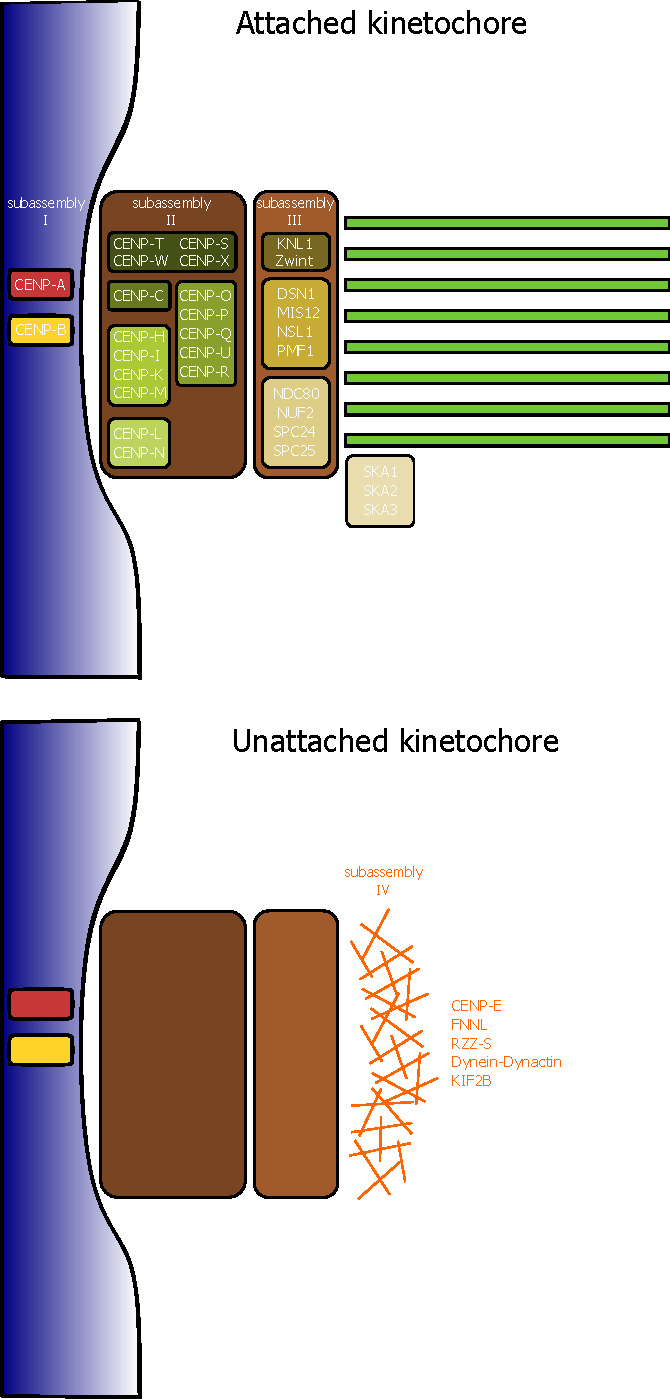
\includegraphics[width=0.9\textwidth]{chapter1/figures/kinetochore.pdf}
  \caption[Schematics of human kinetochore]{Schematics of human kinetochore. The human kinetochore is divided into four subassemblies as described by \citep{McAinsh2022TheKinetochores}. Moving away from centromeric chromatin, subassembly I contains CENP-A and CENP-B. Subassembly II, the inner kinetochore, consists of five subcomplexes, namely CENP-C, CENP-LN, CENP-HIKM, CENP-TWSX and CENP-OPQUR. Subassembly III, the outer kinetochore, is composed of KNL1, MIS12, NDC80 and SKA complexes. On unattached kinetochores, subassembly IV, the corona, forms, which comprises CENP-E, FNNL complex, RZZ-S complex, dynein-dynactin and KIF2B. }
  \label{fig:KTSchematics}
\end{figure}

In human cells, subassembly II, or the CCAN, is composed of 16 different proteins and can be further divided into five subcomplexes. Central to its assembly is CENP-C. Although classified in subassembly II, CENP-C is recognised as the 'blueprint' of the whole kinetochore because it sequentially, from N- to C-terminus, contains a MIS12 complex (assembly III) binding site, CCAN subcomplexes (assembly II) binding sites and CENP-A nucleosomes (assembly I) binding sites. With the scope of CCAN, CENP-C interacts with CENP-HIKM and CENP-LN. Recent cryo-EM data on human CCAN bound to a CENP-A nucleosome revealed that, alongside the CENP-A nucleosome, the CCAN excluding CENP-C forms a gate-like structure wrapping the linker DNA, with CENP-C connecting the two structures. Within the gate-like structure, CENP-OPQUR and CENP-HIKM formed two pillars; CENP-LN formed the arc and CENP-TWSX formed the base \citep{Yatskevich2022StructureNucleosome}. Despite the low level of sequence conservation, budding yeast CCAN, Ctf19 complex, indicated a highly similar structure to human CCAN by cryo-EM, suggesting a potential generality of eukaryotic kinetochore assembly principles. However, the importance of the CCAN is compromised by the non-essentiality of the components. In budding yeast, only 3 out of 14 components are required for cell viability. In human cells, variable results existed due to the acuteness and completeness of protein depletion and the types of cells used. This might have evolutionary indications, such as that the complexity of the network allowed a large degree of freedom and led to the flexibility in the requirement of a certain protein for a certain function among organisms. 

Sometimes referred to as the KMN-S network, subassembly III is built from four subcomplexes, KNL1, MIS12, NDC80 and SKA complexes. It is localised on subassembly II, the inner kinetochore, facing the opposite direction of DNA, hence is also called the outer kinetochore, and directly mediates the interaction between the kinetochore and microtubules. The KNL1 complex is the signalling hub of the cell cycle checkpoint monitoring the status and correctness of kinetochore-microtubule attachment, which is termed SAC and will be introduced in Chapter 1.3.1. It is a heterodimer composed of KNL1 and ZWINT, with the structure and function of the former well studied whereas that of the latter largely remained unknown. From N- to C-terminus, the KNL1 protein possesses a PP1 binding motif that might be under the phospho-regulation by Aurora B, MELT motifs whose phosphorylation by MPS1 forms docking sites for the key SAC signalling proteins BUB1-BUB3 complex, which then recruits MAD1-MAD2 complex and BUB3-BUBR1-PP2A complex, a ZWINT-binding motif predicted to form a coiled-coil structure and RWD domains interacting with the stalk of MIS12 and NSL1. The delicate interplay among kinases and phosphatases present on KNL1 is central to SAC signalling. The MIS12 complex forms the linkage connecting subassembly II and the other subcomplexes of subassembly III. Four structural paralogs, DSN1, MIS12, NSL1 and PMF1, compose the Y-shaped complex. The tips of the Y interact with the CCAN  while the stalk binds both the KNL1 and NDC80 complexes. The interaction between the MIS12 complex and CCAN relies on the direct binding of MIS12 protein to CENP-C, which requires the phosphorylation of DSN1 by Aurora B which exposes the binding site. This requirement has been proposed to prevent kinetochore assembly by non-centromeric CENP-C. The NDC80 complex, together with the SKA complex, is responsible for the capture of spindle microtubules. It consists of an NDC80-NUF2 and an SPC24-SPC25 heterodimer. The two dimers possess a very similar structure composed of a globular head and a coiled-coil stalk, except that NDC80-NUF2 has a break in the stalk, which is believed to provide rotational freedom. The SPC24-SPC25 dimer binds both the MIS12 complex and the CCAN through the interaction between its RWD domains and MIS12 protein or CENP-T. On the opposing end, the CH domain of the NDC80-NUF2 dimer mediates the interaction with microtubules. The NDC80 complex undergoes jackknifing in the absence of microtubule binding. Evidence has been reported linking this conformational change to the attachment-sensing function of SAC. In metazoa, subassembly III of attached kinetochores further contains the SKA complex to enhance microtubule binding. The SKA complex is a W-shaped complex dimerised from trimers comprising SKA1, SKA2 and SKA3, with the microtubule-binding domain of SKA1 located at the tip of the W. The interaction between SKA3 and coiled coils of the NDC80 complex has been shown to facilitate microtubule binding. Although lacking direct orthologs, budding yeast has a functional equivalent to the SKA complex, named the Dam1 complex. It is a heterodecamer that is able to assemble a ring-like structure with other fifteen copies. Two Dam1 complex rings are present on each kinetochore. Similar to the SKA complex, the DAM1 complex associates with the kinetochore in the presence of microtubules and strengthens their interactions. 

kinetochore subassembly IV
kt and peri-cen chromatin structure

\nomenclature{ICEN}{Interphase CENtromere complex}
\nomenclature{KMN-S}{Knl1, Mis12, Ndc80 and Ska}
\nomenclature{RZZ-S}{Rod-Zw10-Zwilch-Spindly}
\nomenclature{FNNL}{CenpF-Nde1-Ndel1-Lis1}
\nomenclature{EM}{Electron Microscopy}
\nomenclature{MELT}{methionine (M)-glutamic acid (E)-leucine(L)-threonine(T)}
\nomenclature{RWD}{RING finger-containing proteins, WD repeat-containing proteins, and DEAD (DEXD)-like helicases}
\nomenclature{CH}{Calponin Homology}


\section{The function of centromere}
\subsection{Error-free kinetochore-microtubule attachment}
\subsection{Robust peri-centromeric cohesion}
\subsection{Advanced replication timing}
\subsection{Chromosome condensation initialisation}
\section{Aims of this study}
\subsection{Building a theoretical model for centromere spatial organisation and propagation}
\subsection{Investigating the molecular mechanisms of tension-dependent re-localisation of shugoshin}
